\documentclass[9pt,twocolumn,twoside]{../../styles/osajnl}
\usepackage{fancyvrb} \journal{i524}

\title{Apache Beam (Google Cloud Dataflow)}

\author[1]{Leonard Mwangi}

\affil[1]{School of Informatics and Computing, Bloomington, IN 47408,
  U.S.A.}

\affil[*]{Corresponding authors: lmwangi@iu.edu}

\dates{\today}

\ociscodes{Cloud, I524, Apache Beam, Google Cloud Dataflow}

% replace this with your url in github/gitlab
\doi{\url{https://github.com/lmundia/sp17-i524/tree/master/paper1/S17-IO-3013/report.pdf}}


\begin{abstract}

  Data has continued to grow in an exorbitant rate and consumers are
  now demanding real-time analytics for answers in order to make
  timely decisions, this has been challenging with batch-based systems
  due to unordered and unbounded dataset being generated and consumed
  thus requiring a paradigm shift to make it possible accommodate
  these datasets.  This paper introduces Apache Beam previously Google
  Cloud Dataflow, a unified model for building data processing
  pipelines that handle both batch and stream processes for bound and
  unbound data.
\newline
\end{abstract}

\setboolean{displaycopyright}{true}

\begin{document}

\maketitle

\section{Introduction}

In the last two decades, there has been a continuous data explosion in
every organization causing them to rethink how to store and make it
consumable so as to gain competitive edge without losing focus to the
core business. This explosion is expected to continue accelerating
with an estimated growth of 4300\% by the year 2020 \cite{www.bigdata}
thus becoming prudent for these organizations to identify solutions
that will help keep this growth at bay and get actionable insights out
of it. There are many solutions in the market that currently solve
this growth and produce useful insights, MapReduce
\cite{www-mapreduce}, Apache Spark \cite{www-spark} and Flink
\cite{www-flink} being some of the leading ones though they have some
major shortcomings. These technologies require either hardware
upgrades \cite{www-upgrademr} or rewriting pipelines to adopt
engine-specific APIs which leads to throw away code especially when
different stream or batch processing is involved. Google Cloud
Dataflow offers an alternative to these technologies allowing you to
run different types of analysis in a cost friendly manner.  Cloud
Dataflow is a fully managed service for creating data pipelines that
ingest, transform and analyze data in both batch and stream mode
\cite{www-streammode}. Based on Millwheel \cite{millwheel} and Flume
\cite{www-flume} technologies, it’s posed as the successor of
MapReduce and allows analysis of large volumes of data real-time in
the cloud thus removing the need for deployment, maintaining and or
scaling infrastructure.  Cloud Dataflow has been submitted and
accepted to Apache incubator, the project is now referred to as Apache
Beam \cite{www-beamincubate}.

\section{Implementation}

Cloud Dataflow is language agnostic, it’s first SDK was written in
Java \cite{www-javasdk} but now available in Python
\cite{www-pythonsdk} allows an entire pipeline to be written in a
single program using intuitive Cloud Dataflow constructs to express
application semantics \cite{www-dataflowconstructs}. The SDKs are
portable allowing it to produce programs that can execute in many
pluggable environments using “runners” which connect to the execution
engines. At the moment, pluggable “runners” exist for Artisan, Apache
Spark, single-node local execution runner by Google and Google hosted
cloud Dataflow service execution engines

Figure \ref{fig:false-color}

\begin{figure}[htbp]
\centering
\fbox{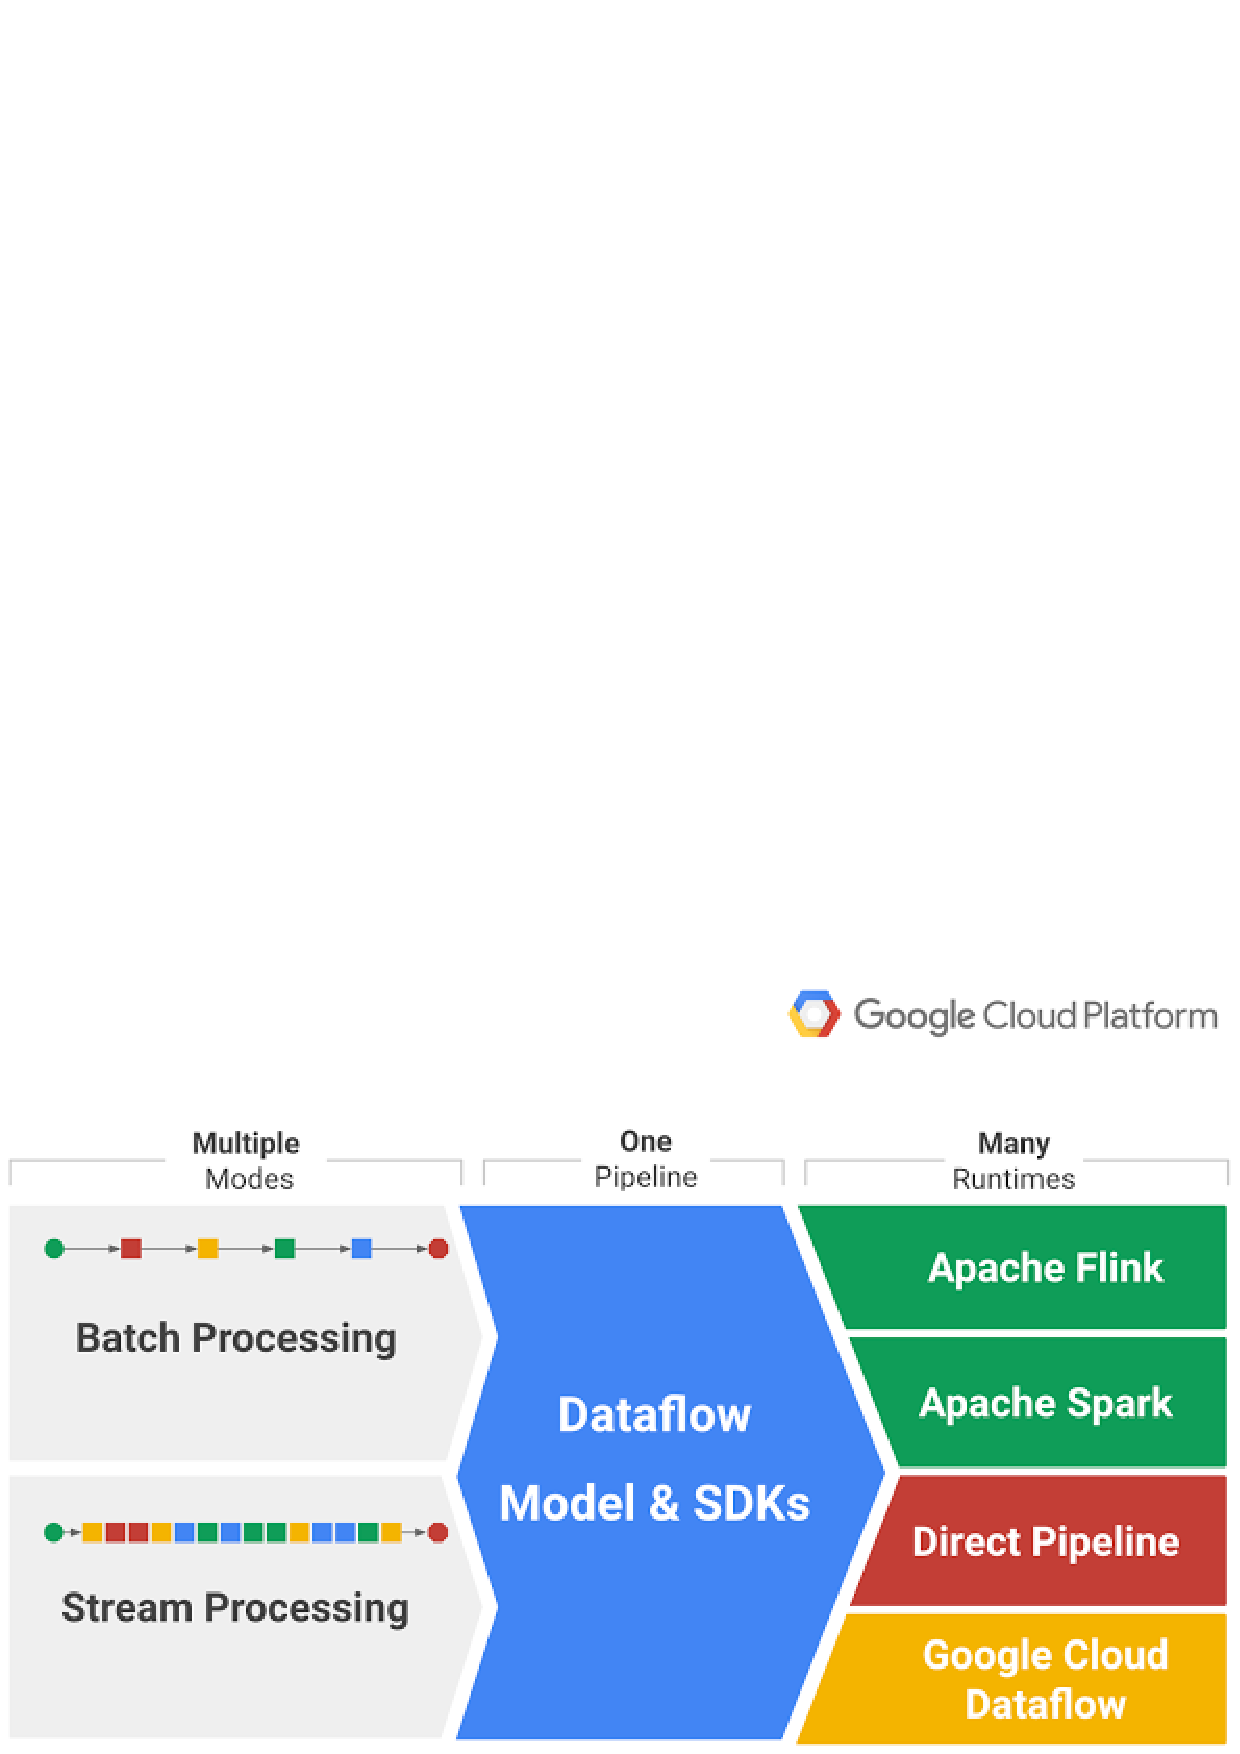
\includegraphics[width=\linewidth]{images/sdkstructure}}
\caption{Dataflow Execusion Engine \cite{www-beamincubate}}
\label{fig:false-color}
\end{figure}

When programing with Dataflow SDK, you essentially create a data
processing job to be executed by one of the runner services. The model
handles the low-level details like coordinating individual workers,
sharding data sets amongst other tasks allowing focus to be on logical
composition of data processing job.

\subsection{Dataflow SDK}

There are four major concepts in Dataflow SDK \cite{www-sdkmodel}:

\begin{itemize}
\renewcommand{\labelitemi}{\scriptsize$\square$}

\item Pipelines – computation process that accepts data input from
  external sources, transforms it to provide some useful intelligence
  and produce some output data.
\item PCollection–represents data in the pipeline, PCollection classes
  can represent virtually unlimited data set size.
\item Transforms – it’s the dataprocessing operation in the pipeline
  taking data from PCollection and producing output PCollection.
\item I/O Sources and Sinks – provides data source and data sink APIs
  for pipeline I/O. Source API reads data into the pipeline and sink
  API writes output data from the pipeline. The source and sink
  represents root and endpoints of a pipeline.
  
\end{itemize}

In order to work with data in the pipeline, it has to be in form of
PCollection. Each PCollection is owned by a specific pipeline object
and only that Pipeline. PCollection has the following limitations:

\begin{itemize}
  \renewcommand{\labelitemi}{\scriptsize$\square$}
  
\item It’s immutable, once created you cannot add, remove, or change
  individual elements
\item It does not support random access to individual elements
\item Cannot be shared between Pipeline objects

\end{itemize}

\subsection{Dataflow SDK}

As mentioned at the beginning of the paper, Cloud Dataflow was
submitted for incubation to Apache and now the project is referred to
as Apache Beam. Thus, in the example below Apache Beam is referenced.

\begin{figure}[htbp]
\centering \fbox{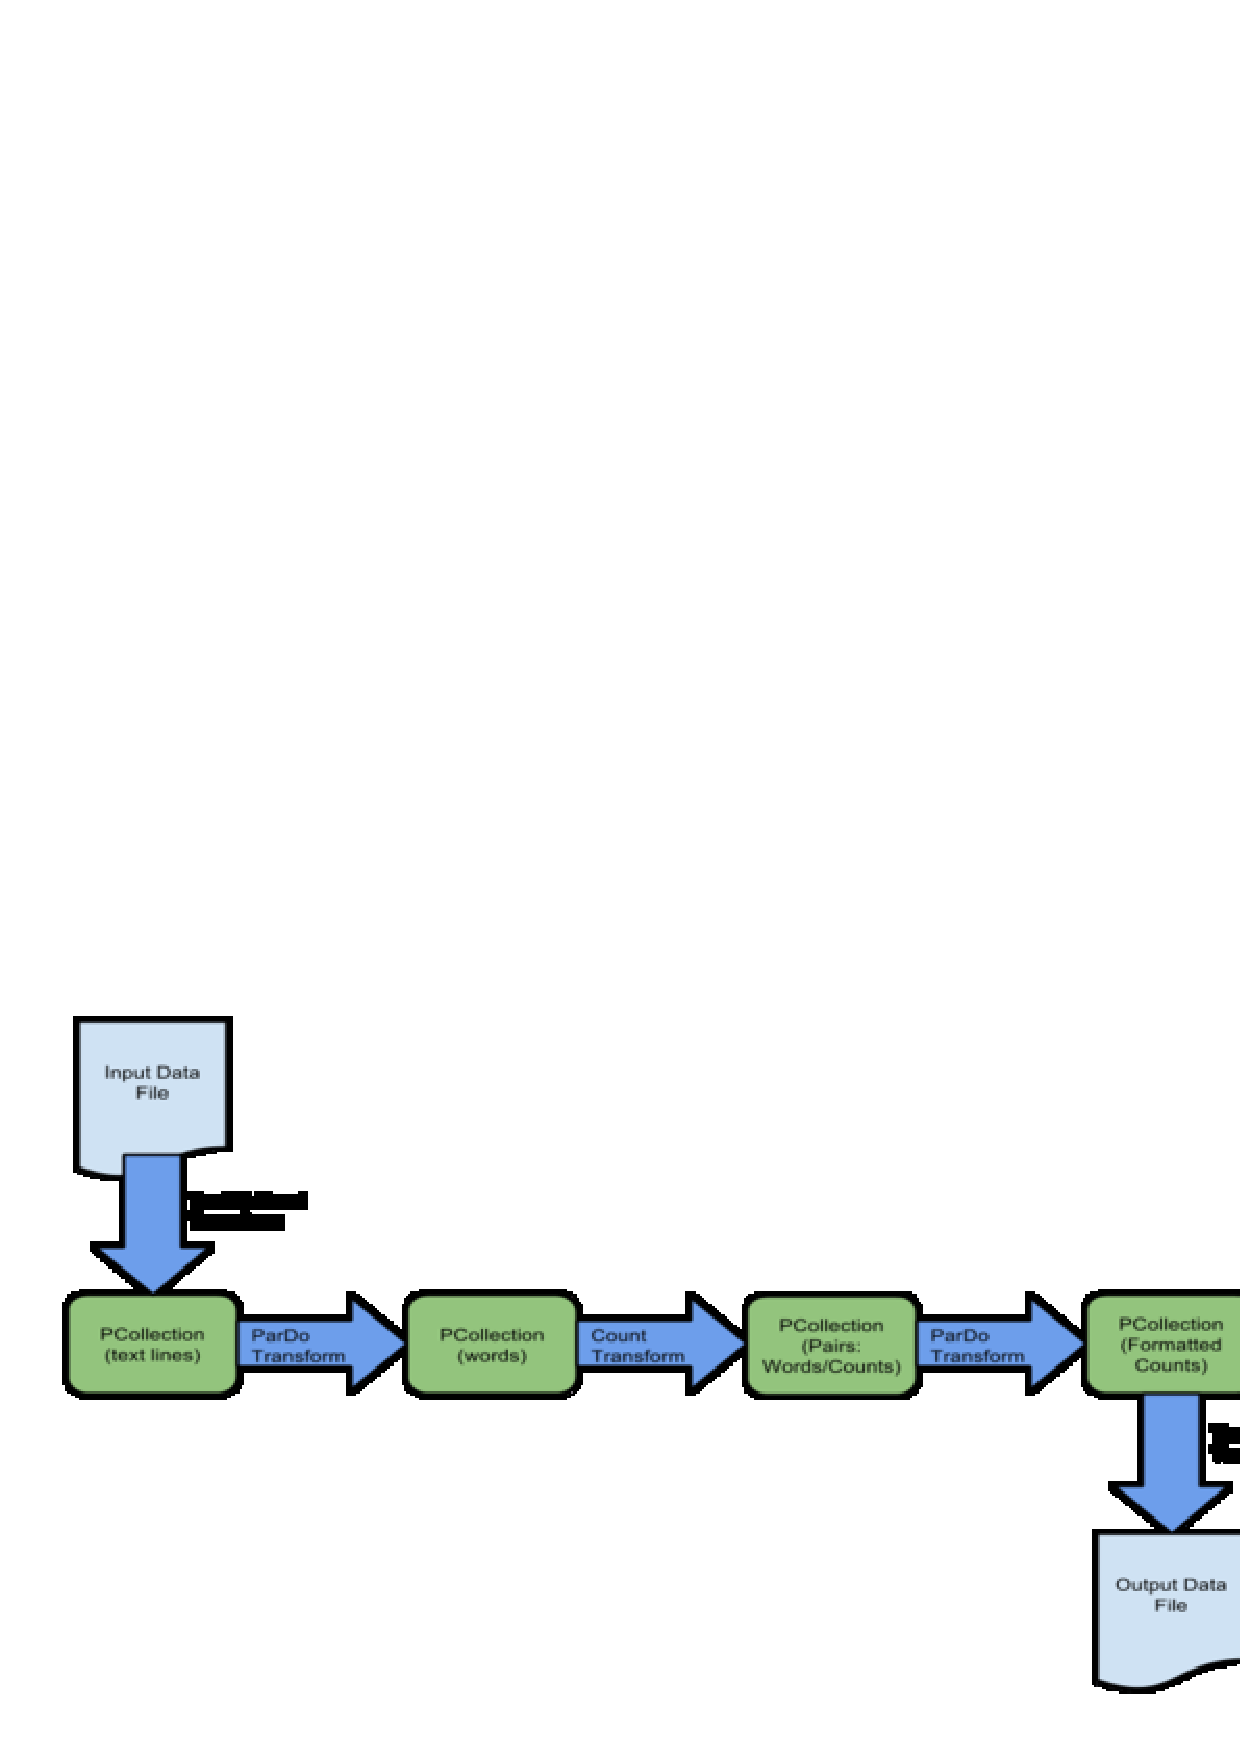
\includegraphics[width=\linewidth]{images/dataflow}}
\caption{Apache Beam dataflow \cite{www-wordcountflow}}
\label{fig:false-color}
\end{figure}

Below is the processing pipeline code, which is accomplishable with a
few lines of code.

\begin{figure}[htb]
\begin{quote}
\begin{Verbatim}
    
# ... other imports ...
import google.cloud.dataflow as df

@df.typehints.with_output_types(df.typehints.Tuple[int,
  float])
def parse_sales_record(line):
  # Lines look like this:
# {"Timestamp": 1234.56, "Price": 10, "ProductName":
  "Name", "ProductID": 4}
record = json.loads(line)
return int(record['ProductID']), float(record['Price'])

p = df.Pipeline(...options...)
(p
| df.io.Read(df.io.TextFileSource('gs://SOMEBUCKET/
PATH/*.json'))
    | df.Map(parse_sales_record)
    | df.CombinePerKey(sum)
    | df.Map(lambda (product, value): {'ProductID':
      product,'Value': value})
    | df.io.Write(df.io.BigQuerySink('SOMEDATASET.
    SOMETABLE'
        schema='ProductID:INTEGER, Value:FLOAT',
        create_disposition=df.io.BigQueryDisposition.
        CREATE_IF_NEEDED,
        write_disposition=df.io.BigQueryDisposition.
        WRITE_TRUNCATE)))
p.run() \end{Verbatim}
\end{quote}
\caption{Processing Python Pipeline Code \cite{www-pythoncode}}\label{alg:python}
\end{figure}

\section{Relation to Big Data}

Collecting, transforming and analyzing big data in near real-time has
become essential as form of getting instant feedback in order to solve
customer needs or solve a problem quickly. Cloud Dataflow provides
that capability through its real-time streaming platform. Cloud
Dataflow allows processing of unbound, out-of-bound and global scale
data \cite{www-statefulprocess}.

\section{Use Cases}

\subsection{Financial Industry}

With constant threats in financial industry, detecting and identifying
anomalies in data flow is paramount to prevent fraud and financial
crimes. By leveraging Cloud Dataflow real-time streaming, the industry
can identify anomalies and notify necessary authorities for further
investigations thus preventing catastrophic outcome.

\subsection{Improve store layout}

Sales are attributed to customers traffic, understanding the behavior
of the customers when they are in a store and re-aligning to cater
their needs helps increase sales. After Capturing these behaviors by
use of RFIDs and QR code sensors, store owners can utilize Cloud
Dataflow to analyze them in real-time and offer incentives like
instant coupons to drive sales \cite{www-storelayout}.

\subsection{Sentiments Tracking}

Every organization wants to know what their customers think about them
and social media makes it easy for the customers to express themselves
on how they feel about a brand. Collecting, quantifying and analyzing
these sentiments becomes daunting task due to large amounts of
data. Cloud Dataflow eases this task due to its ability to stream and
analyze real-time data. Cloud Dataflow taps into social media outlets
and analyzes the sentiments thus giving the organization a clear
picture in real-time of what customers think and can also be used to
re-align the marketing message for a better outcome.

\section{Alternative Technologies}

\subsection{Amazon Kinesis Stream}

Amazon Kinesis Stream is an AWS data streaming offering that can
capture and analyze data from different sources in real-time
\cite{www-kinesis}. Using Kinesis Client Library (KCL) developers have
the ability to write Amazon Kinesis powered applications that can
generate and store data in other AWS offerings. A subscription is
required in order to use Kinesis Stream. In comparison to Cloud
Dataflow, Kinesis Stream has a limitation of 1MB/sec while Cloud
Dataflow has a limitation of 10MB also Kinesis deployment locality is
limited to regional while Dataflow is global \cite{www-awscomparison}.

\subsection{Azure Stream Analytics (ASA)}

Like Cloud Dataflow, Azure Stream Analytics is a fully managed
real-time event processing engine capturing data from different
sources and provide analytics [www-asa]. Stream Analytics is provided
through Azure portal where analytics jobs can be authored. Stream
Analytics connectivity is limited to Azure platform [www-asa] whereas
Cloud Dataflow runners integrate with Flink, Spark and local runners
for testing.

\subsection{Apache Spark}

Apache Spark also a competing solution to Cloud Dataflow, is a fast
in-memory data processing engine with expressive development APIs that
allow data workers to efficiently execute streaming, machine learning
or SQL workloads \cite{www-spark}. The downside to Spark is that it’s
a batch-based processing framework \cite{www-notstream} thus limiting
true record-by-record processing also data arriving out-of-sequence
possess a problem because it may be processed in the wrong batch.

\section{Conclusion}

Data growth is going to continue by staggering numbers and the
consumers are becoming more aware of what they can accomplish with it
thus demanding powerful platforms that can cater their needs as close
to real-time as possible. Google Cloud Dataflow offers the solution to
these needs by providing a stream and batch processing model thus not
limiting the type of data being consumed. Making Cloud Dataflow
available as an Apache Project increases reachability and enhances
visibility to allow more runners to be incorporated to project. With
more runners, it becomes cheaper and easier to migrate the existing
on-premise and cloud solutions to Cloud Dataflow (Apache Beam) that
may benefit from its processing capabilities.  By handling the
low-level details tasks in the system, Dataflow allows the developers
to focus on the core processes of the pipeline which generates the
desired performance, reliability and correctness. This makes Cloud
Dataflow very attractive platform to handle big data needs.

\section{Acknowledgement}

This research was done as part of course “I524: Big Data and Open
Source Software Projects” at Indiana University. I thank Professor
Gregor von Laszewski and associate instructors for their support
throughout the course.

% Bibliography

\bibliography{references}
 
\end{document}
